\subsection{Discussion}
This project served as a foundation to enable future research and testing.
This framework is going to be used more as a testing environment for future work such
as multiagent micromouse simulation in a realistic 3d environment allowing the user to easily test
their Algorithms, with sensing and realistic robot maneuvering. Before this system is launched
we will provide a more robust steering mechanissdm which will take into account the robot model,
this will abstract out the difficulty associated with navigating to a goal or following a line.
In addition to abstracting out the motion models, this framework is designed to support complex
multiagent decision making like those represented in behavioral trees.

robots to share their information states including the enountered
terrain in order for the robot team to best explore and traverse a
given heterogenous environment. The resultant decision that is derived
from an agents neighbor's states namely TREE STATE, this variable
represents the robots decision, which could entail further investigation
(PROD) or stopping all motion and entering into a low power mode (IDLE).


\begin{figure}[H]
  \centering
    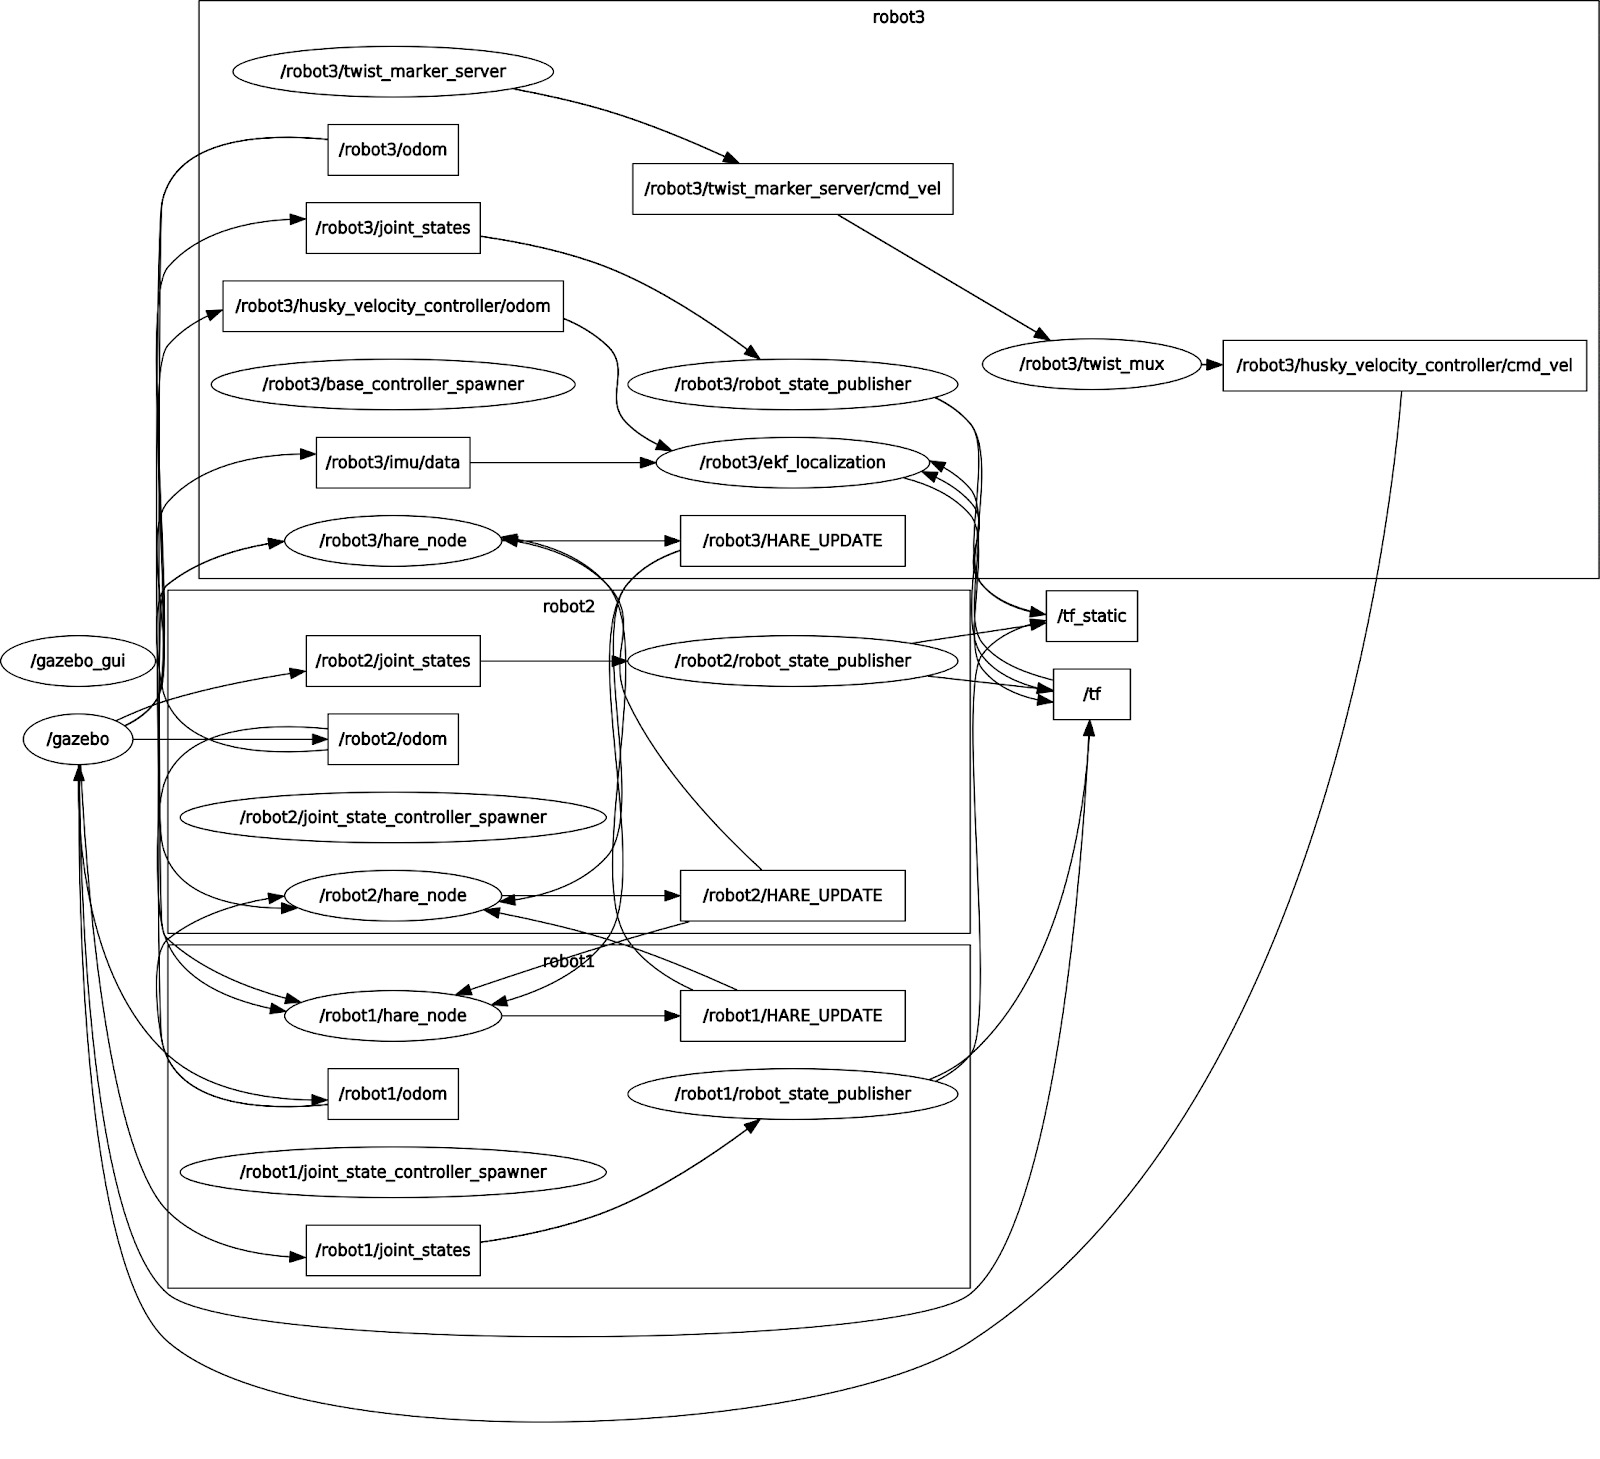
\includegraphics[width=0.4\textwidth]{rqt-graph}
  \caption{ROS multi-master communication architecture}
  \label{fig:comm}
\end{figure}

\subsection{Future Work}
Even though the testing framework was not the overall goal of this research,
it turned out to be one of the strong suits of the project. Future work would certainly
include iteration on this framework to ensure that it is as easy as possible to
randomly generate maps as well as add any number of any kind of robot. The benefit
of doing this on Gazebo is the ability to emulate robotic agents much closer to the
real world representation than Unity, ARGoS, or any other open source platform
capable of multi-robot simulation. Another step would ofcourse be iteration of the tested cooperation model on hardware.
This would require much more extraneous simulation to ensure that all edge cases are
covered. To properly do this, the testing framework would have to be iterated as
described above. Due to Gazebo not inherently supporting multimaster network architectures,
there is the possibility that a plugin or new simulation package would need to be
developed \cite{ROS-mm}. The communication architecture with all nodes encapsulated within the robot namsepace
this communication archietecture is shown in figure \ref{fig:comm}.
